\documentclass{beamer}
\usetheme{Madrid}
\usecolortheme{beaver}
\usepackage{graphicx}
\usepackage{booktabs}
%-------------------------------------------------
\author{Vyshak Puthusseri} 
\date{23th Oct 2019}
\institute[CET]
{
College of Engineering, Trivandrum\\\\
\text{TVE17MCA054}
}

\title{STYLE GAN : A Style Based Generator Architecture for Generative Adversarial Networks}
%-------------------------------------------------



\setbeamertemplate{footline}
{
  \leavevmode%
  \hbox{%
  \begin{beamercolorbox}[wd=.5\paperwidth,ht=2.25ex,dp=1ex,center]{author in head/foot}%
    \usebeamerfont{author in head/foot}\insertshortauthor
    
  \end{beamercolorbox}%
  \begin{beamercolorbox}[wd=.5\paperwidth,ht=2.25ex,dp=1ex,center]{title in head/foot}%

    \insertframenumber{} / \inserttotalframenumber\hspace*{1ex}
  \end{beamercolorbox}}%
  \vskip0pt%
}


\begin{document}
\titlepage 
\begin{frame}
    {Introduction}
    \tableofcontents   
\end{frame}

\section{Deep Learning}
\section{GAN : Generative Adversarial Network}
\section{Style Transfer}
\section{Style Based Generator Architecture for GAN}
\section{Conclusion}
\section{References}

\chapter{Deep Learning}
\par
    Deep learning is an artificial intelligence function that imitates the workings of the human brain in processing data and creating patterns for use in decision making. Deep learning is a subset of machine learning in artificial intelligence (AI) that has networks capable of learning unsupervised from data that is unstructured or unlabeled. Also known as deep neural learning or deep neural network. The basic building block of a neural network is known as LTU(Linear Threshold Unit). LTU was only a concept. There will be no learning rule for an LTU. If we apply a learning rule to the architecture it is known as perceptron. It will have a step activation function. SO only binary classifica

%%%%%%%%%%%%%%%%%%%%%%                                          About Style Transfer
\begin{frame}[fragile]{Neural Style Transfer}
   Style transfer relies on separating the content and style of an image. 
   \\
   Given one content image and one style image, we aim to create a new, target image which should contain our desired content and style components:
    \begin{itemize}
        \item feature reconstruction
        \item texture synthesis
    \end{itemize}

\end{frame}


%%%%%%%%%%%%%%%%%%%%%%                                         
\begin{frame}[fragile]{Neural Style Transfer}
    \begin{equation}
        content.image + style.image =  new.image with style.transfered
    \end{equation}
    \begin{figure}[ht]
      \hspace*{-1cm}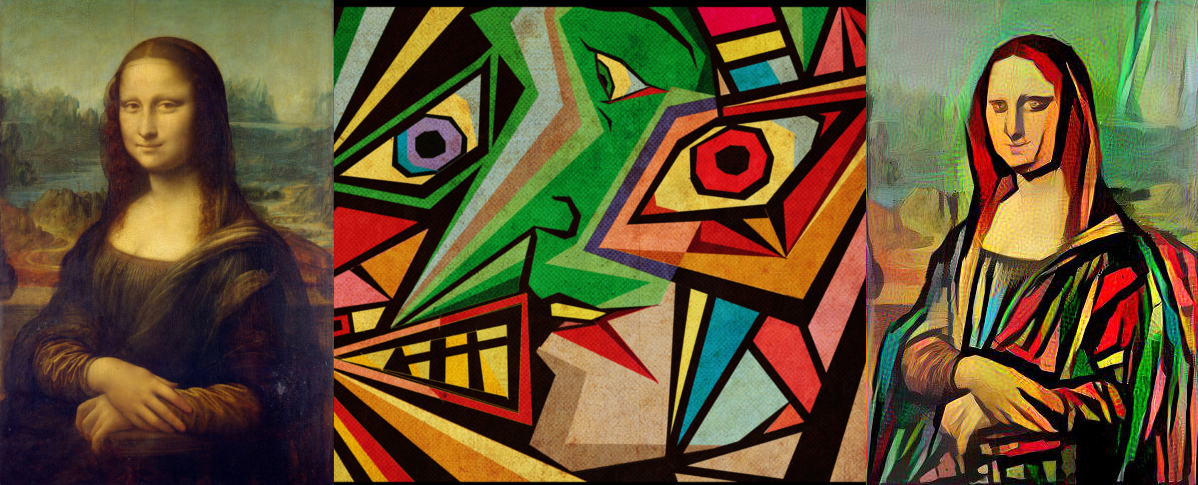
\includegraphics[width=0.5\linewidth]{styletransfer} \\
      \hspace*{-1cm}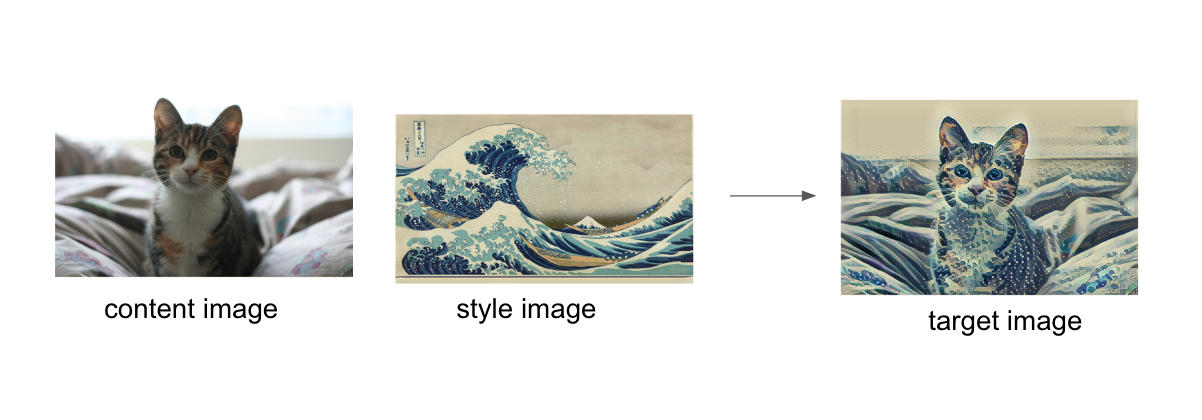
\includegraphics[width=0.7\linewidth]{styletransfercat} 
    \end{figure}
    https://github.com/puthusseri/styleTransfer.git
\end{frame}


%%%%%%%%%%%%%%%%%%%%%%%%%%%%%%%%%%%%%%%%%%%%%%%%%%


%%%%%%%%%%%%%%%%%%%%%%                                          About GAN                    
\begin{frame}[fragile]{Generative Adversarial Network}
 GANs are generative models: they create new data instances that resemble your training data. \\
 eg: images that look like photographs of human faces, even though the faces don't belong to any real person.
     \begin{figure}[ht]
      \hspace*{-1cm}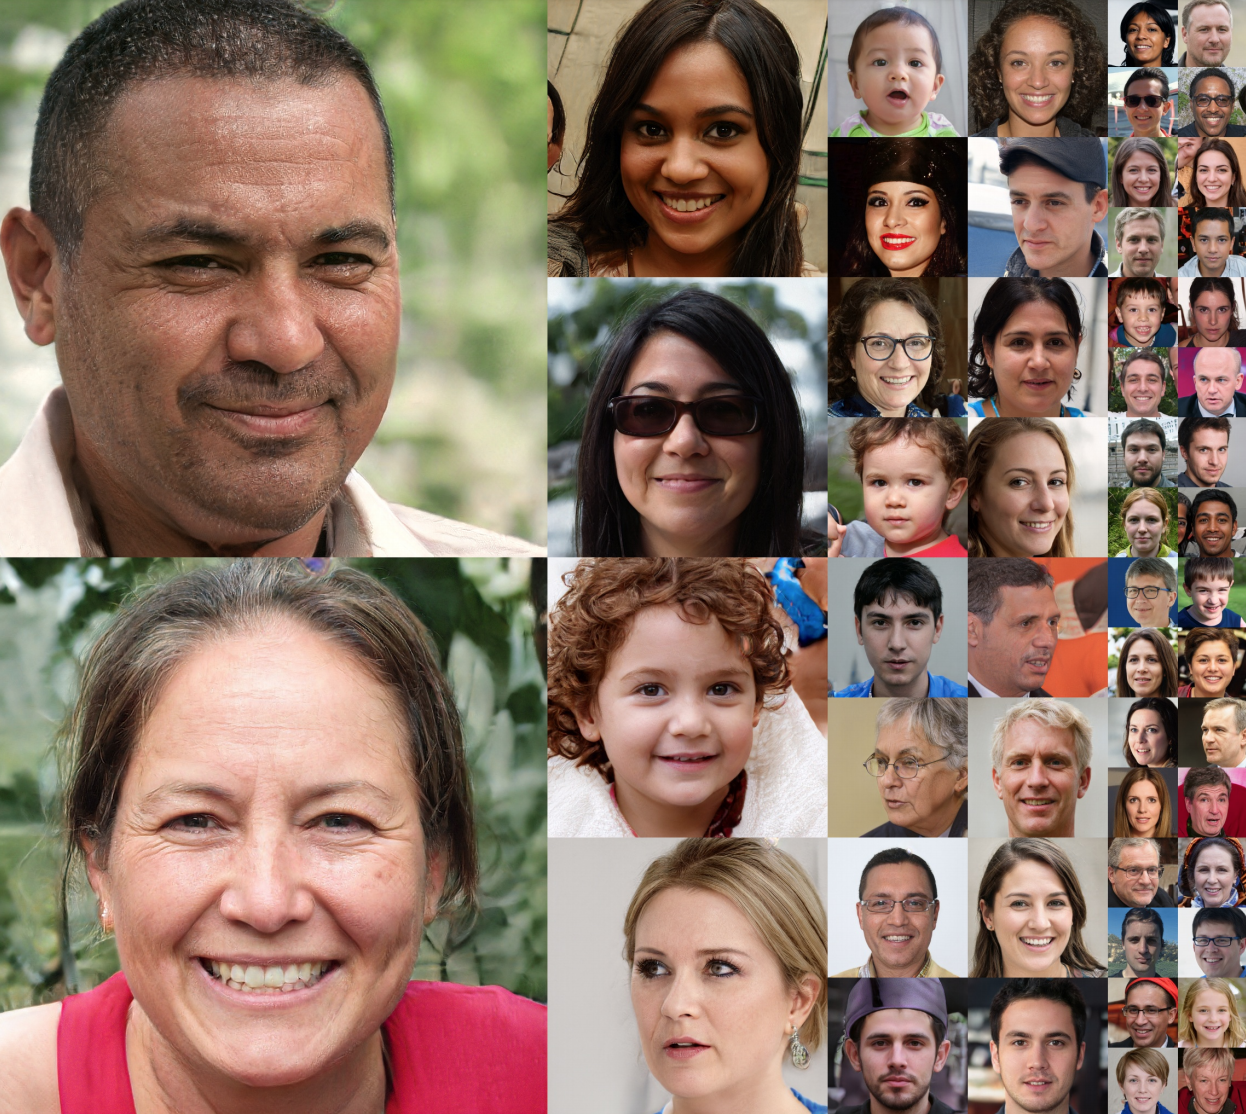
\includegraphics[width=0.5\linewidth]{ganhumans} 

    \end{figure}
\end{frame}

%%%%%%%%%%%%%%%%%%%%%%                                          About GAN Applications                   
\begin{frame}[fragile]{GAN : Applications}

    \begin{itemize}
        \item Image to image translation (in unsupervised way)
        \item blue prints to real image
        \item photo to cartoon (Facebook AI research)
        \item photo of day to night (NVIDIA Research)
        \item Creating stimulated training set (eg : face recognition problem)
        \item for imitaion learning
    \end{itemize}
\end{frame}

%%%%%%%%%%%%%%%%%%%%%%                                          About GAN Overview                   
\begin{frame}[fragile]{GAN : Overview}
 GANs has two parts: \\
    \begin{itemize}
        \item The generator : learns to generate plausible data. The generated instances become negative training examples for the discriminator.

        \item The discriminator: learns to distinguish the generator's fake data from real data. The discriminator penalizes the generator for producing implausible results.
    \end{itemize}
\end{frame}


%%%%%%%%%%%%%%%%%%%%%%                                          About GAN Training                   
\begin{frame}[fragile]{GAN : Training}
     \begin{figure}[ht]
         \hspace*{-1cm}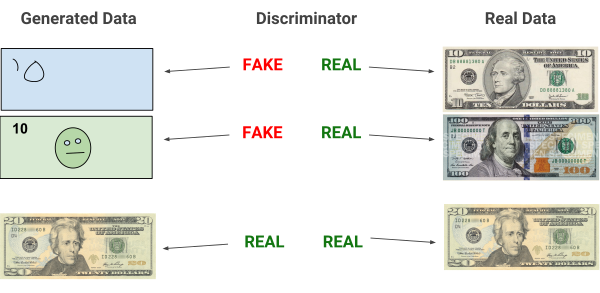
\includegraphics[width=0.7\linewidth]{gantrain} \\ \\ \\ \\ \\ 


    \end{figure}
\end{frame}

%%%%%%%%%%%%%%%%%%%%%%                                          About GAN Architecture                   
\begin{frame}[fragile]{GAN : Architecture}
     \begin{figure}[ht]
         \hspace*{-1cm}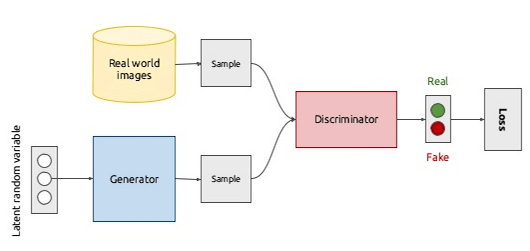
\includegraphics[width=0.7\linewidth]{ganarchitecture.png} \\ \\ \\ \\ \\ 
    \end{figure}
\end{frame}
%%%%%%%%%%%%%%%%%%%%%%%%%%%%%%%%%%%%%%%%%%%%%%%%%%%%%%%%%%%%%%%%%%%%%%

%%%%%%%%%%%%%%%%%%%%%%                                          About Style Based GAN                   
\begin{frame}[fragile]{Style Based GAN}
        \begin{itemize}
        \item Introduced by NVIDIA 
        \item Improved the efficiency of GAN by improving the generator
        \item Introduced new automated metrics - perceptual path length and linear seperability
        \item Result was  : new dataset Flickr Face HQ (FFHQ) of size 2.56 TB
    \end{itemize}

\end{frame}

%%%%%%%%%%%%%%%%%%%%%%                                          About Style Based Generator                   
\begin{frame}[fragile]{Style Based Generator}
        \begin{itemize}
        \item The weights are studied through the 8 layer affine transformation.
        \item Feature maps are normalized using AdaIN
        \item Generate \textit{stochastic details} by introducing the explicit noise for each layer.
        \item Final resulting feature maps are passed to the discriminator.
    \end{itemize}

\end{frame}

%%%%%%%%%%%%%%%%%%%%%%                           About Style Based Generator Architecture                   
\begin{frame}[fragile]{Style Based Generator : Architecture}
     \begin{figure}[ht]
         \hspace*{-1cm}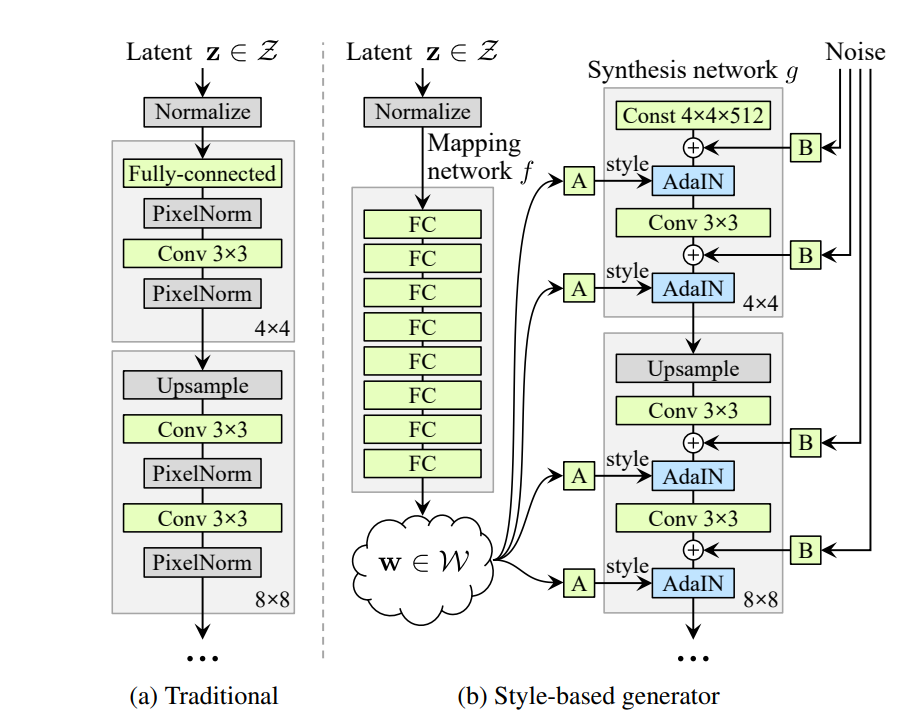
\includegraphics[width=0.9\linewidth]{styleganarchitecture.png} \\ \\ \\ \\ \\
    \end{figure}
\end{frame}

%%%%%%%%%%%%%%%%%%%%%%                                          About Style Based Image Quality                   
\begin{frame}[fragile]{Image Quality }
        \begin{itemize}
        \item Comparing with CelebA-HQ with FFHQ based on Frechet inception distances (FID) , a great improvement happens
        \item Used truncation trick
        \item Used 26.3M parameters for training
        \item Generated image is of 1024 * 1024 resolution
    \end{itemize}

\end{frame}

%%%%%%%%%%%%%%%%%%%%%%%%%%%%%%%%%%%%%%%%%%%%%%%%%%%%%%%%%%%%%%%%%%%%%%

%%%%%%%%%%%%%%%%%%%%%%                                  About Style Based generator Properties  1                 
\begin{frame}[fragile]{Style Based Generator : Properties }
        \begin{itemize}
        \item Style mixing - mixing regularization
    \end{itemize}
    \begin{figure}[ht]
         \hspace*{-1cm}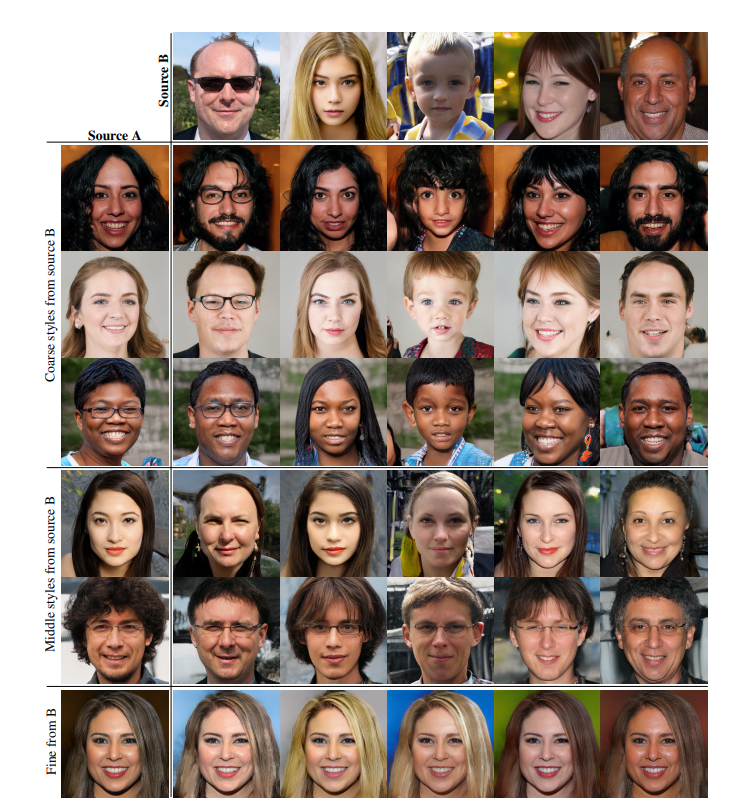
\includegraphics[width=0.6\linewidth]{stylemixing.png} \\ \\ \\ \\ \\
    \end{figure}

\end{frame}

%%%%%%%%%%%%%%%%%%%%%%                                  About Style Based generator Properties  2                
\begin{frame}[fragile]{Style Based Generator : Properties }
        \begin{itemize}
        \item Stochastic variation
    \end{itemize}
    \begin{figure}[ht]
         \hspace*{-1cm}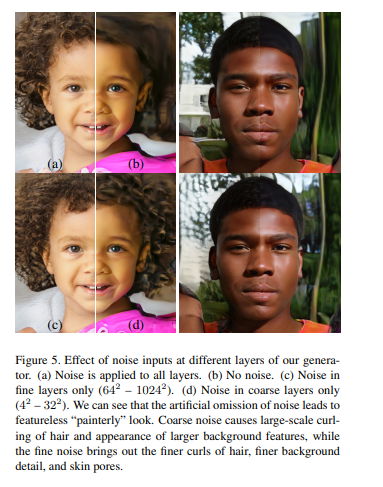
\includegraphics[width=0.7\linewidth]{stochasticvariation.png} \\ \\ \\ \\ \\
    \end{figure}

\end{frame}

%%%%%%%%%%%%%%%%%%%%%%%%%%%%%%%%%%%%%%%%%%%%%%%%%%%%%%%%%%%%%%%%%%%%%%


\begin{frame}
  \begin{align*}
    \includegraphics[width=90mm]{gan13}  
\end{align*}  
\end{frame}
\begin{frame}{What is Generative Adversarial Networks (GAN)?}   
\begin{align*}
    \includegraphics[width=90mm]{gan2}  
\end{align*}
\end{frame}
\begin{frame}   
\begin{itemize}
\item The two adversarially trained models are: a generative
model G and a discriminative model D.
\item The generator G takes a latent variable z as input, and outputs sample G(z).
\item The discriminator D takes a sample x as input and outputs
D(x) which represents the probability that it is real.
\item The \underline{training procedure} is similar to a two-player min-max game
with the following objective function:

\begin{align*}
    \includegraphics[width=100mm]{gan3}  
\end{align*}
\end{itemize}

\end{frame}
%----------------------------------------------------------------
\section{Socially-Aware GAN}
\begin{frame}{Solution: Socially-Aware GAN(SGAN)} 
\begin{itemize}
\item \Large Our proposed GAN is a RNN Encoder-Decoder generator and a RNN based encoder discriminator with two novelities:
\begin{itemize}
    \item {\large a variety loss function-adversarial loss}
    \item {\large pooling mechanism - that learns a “global” pooling vector which encodes the actions of all people
involved in a scene}
\end{itemize}
\end{itemize}
\end{frame}
%----------------------------------------------------------------
\begin{frame}{SGAN conti...} 
\begin{itemize}
     \item {\large A} {\LARGE variety loss function}{\large -the distance between the true and the generated distributions at the current iteration.}
\begin{align*}
    \includegraphics[width=60mm]{gan6}  
\end{align*}
\end{itemize}
\end{frame}
%----------------------------------------------------------------
\begin{frame}{SGAN conti...} 
\begin{itemize}
    \item Our model consists of three key components: Generator (G),
Pooling Module (PM) and Discriminator (D).
\item G is based on encoder-decoder framework where we link the hidden
states of encoder and decoder via PM. 
\item G takes as input Xi and outputs predicted trajectory $\hat Yi$. D inputs the entire sequence comprising both input trajectory Xi and future prediction $\hat Yi$ (or Yi) and classifies them as “real/fake”.
\end{itemize}
\begin{align*}
    \includegraphics[width=120mm]{gan5}  
\end{align*}
\end{frame}
%----------------------------------------------------------------
\begin{frame}{SGAN conti...} 
\huge Generator-Encoder
 \begin{itemize}
    \item \large We first embed the location of each person
using a single layer MLP to get a fixed length vector $e^t_{i}$.
These embeddings are used as input to the LSTM cell of the \underline {encoder} at time t introducing the following recurrence:
 \begin{align*}
    \includegraphics[width=50mm]{gan7}  
\end{align*}
where $\phi$(·) is an embedding function with ReLU nonlinearity,
$W_{ee}$ is the embedding weight. The LSTM weights $(W_{encoder})$ are shared between all people in a scene.
 \end{itemize}
\end{frame}

\begin{frame}{SGAN conti...} 
\huge Generator-Decoder
 \begin{itemize}
    \item \large After initializing the \underline {decoder} states as described above we can obtain predictions as follows:
 \begin{align*}
    \includegraphics[width=70mm]{gan8}  
\end{align*}
where $\phi$(·) is an embedding function with ReLU nonlinearity
with $W_{ed}$ as the embedding weights. The LSTM
weights are denoted by $(W_{decoder})$ and is an MLP.
 \end{itemize}
\end{frame}
%----------------------------------------------------------------
\begin{frame}{SGAN conti...} 
\huge Discriminator\\
 \begin{itemize}
    \item \Large The discriminator consists of a separate
encoder. Specifically, it takes as input $T_{real}$ = [Xi, Yi] or
$T_{fake}$ = [Xi,$\hat Yi$] and classifies them as real/fake.
\end{itemize}
\end{frame}
%----------------------------------------------------------------
\begin{frame}{SGAN conti...} 
\huge Pooling Module- \Large Social Pooling\\
 \begin{itemize}
    \item \Large Variable and (potentially) large number of people in a scene. We need a compact representation which combines information from all the people.
    \item \Large Scattered Human-Human Interaction.
    
     \begin{align*}
    \includegraphics[width=90mm]{gan9}  
\end{align*}
\end{itemize}
\end{frame}
%----------------------------------------------------------------
\section{Evaluations}
\begin{frame}{Evaluations} 
\huge Quantitative Evaluation
 \begin{align*}
    \includegraphics[width=120mm]{gan10}  
\end{align*}
\small ADE-Average Displacement Error\\
\small FDE-Final Displacement Error
\end{frame}

\begin{frame}{Evaluations} 
\huge Qualitative Evaluation
 \begin{align*}
    \includegraphics[width=120mm]{gan11}  
\end{align*}

\end{frame}
%----------------------------------------------------------------
\begin{frame}{Evaluations} 
\huge Real World Scenario
 \begin{align*}
    \includegraphics[width=120mm]{gan12}  
\end{align*}
\end{frame}
%----------------------------------------------------------------
\section{Conclusion}
\begin{frame}{Conclusion}
    \begin{itemize}
        \item We tackle the problem of modeling human-human
interaction and jointly predicting trajectories for all
people in a scene.
        \item We propose a novel GAN based encoder-decoder
framework for trajectory prediction capturing the
multi-modality of the future prediction problem.
        \item Introduced pooling mechanism enabling the network to learn social norms.
       \item We saw the efficiency of
our method on several complicated real-life scenarios where
social norms must be followed.


    \end{itemize}
\end{frame}
%----------------------------------------------------------------
\section{References}
\begin{frame}{References}
    \begin{itemize}
        \item Social GAN: Socially Acceptable Trajectories with Generative Adversarial Networks by Agrim Gupta, Justin Johnson1, Li Fei-Fei1 Silvio Savarese,Alexandre Alahi.
        \item A. Alahi, K. Goel, V. Ramanathan, A. Robicquet, L. Fei-Fei, and S. Savarese. Social lstm: Human trajectory prediction in crowded spaces. 
        \item D. Helbing and P. Molnar. Social force model for pedestrian dynamics. 
       \item Analyzing the Variety Loss in the Context of Probabilistic Trajectory Prediction by Luca Anthony Thiede and Pratik Prabhanjan Brahma
\item Other online sources.


    \end{itemize}
\end{frame}
%----------------------------------------------------------------
\begin{frame}
\begin{align*}
    \includegraphics[width=60mm]{thankyou}  
\end{align*}

\end{frame}
\end{document}